\documentclass[11pt]{article}
\usepackage[utf8]{inputenc}
\usepackage[T1]{fontenc}
\usepackage{lmodern}
\usepackage{geometry}
\usepackage{amsmath,amssymb,amsthm}
\usepackage{booktabs}
\usepackage{array}
\usepackage{graphicx}
\usepackage{algorithm}
\usepackage{algpseudocode}
\usepackage{hyperref}
\usepackage{enumitem}
\usepackage{tikz}
\usetikzlibrary{arrows.meta,positioning}
\geometry{margin=1in}
\hypersetup{colorlinks=true,linkcolor=blue,citecolor=blue,urlcolor=blue}

\title{K3M: Compression by Kakeya-Like Support Construction for 3D Perceptual Memory}
\author{
Allen Li \\
\textit{Independent Researcher} \\
\texttt{AllenL329@gmail.com}
\and
GPT-5.4 \\
\textit{AI Research Collaborator}
}
\date{\today}

\newtheorem{definition}{Definition}
\newtheorem{proposition}{Proposition}
\newtheorem{remark}{Remark}

\begin{document}
\maketitle

\begin{abstract}
We propose \textbf{K3M}, a support-first compression framework for 3D perceptual memory inspired by the constructive intuition behind three-dimensional Kakeya-type sets. The motivating principle is that rich directional structure need not occupy large ambient volume. We argue that this principle has a natural compression-theoretic interpretation for long-context memory: the primary object to compress is not a dense tensor of coefficients, but a thin support set carrying the dominant directional content of the data. K3M therefore first constructs a discrete Kakeya-like support inside a 3D memory volume and only then encodes the signal restricted to that support, together with a low-frequency background and a sparse residual. We present the mathematical formulation, a discrete construction mechanism, a runnable Python prototype, and two complementary empirical lenses. On synthetic 3D volumes, K3M exhibits the intended geometric behavior of small active support at competitive recall. On real text-memory benchmarks, we argue that evaluation must separate \emph{retrieval realism} from \emph{perceptual-memory realism}. Using the official AAAK retrieval benchmark and a new PMS-Bench benchmark centered on constraints, turning points, and causal recall, we show that official AAAK remains stronger on classical compression-oriented retrieval, while a support-first \texttt{constraint-edge fixed} K3M-style backend is substantially stronger on perceptual-memory recovery, query latency, and benchmark-native constraint fidelity. These results suggest that Kakeya-like support construction is not merely a geometric compression heuristic, but a plausible organizing principle for memory systems whose value lies in preserving thin, query-useful structural supports rather than only maximizing dense-session retrieval.
\end{abstract}

\section{Introduction}
The central claim of this paper is that the compression-theoretic value of the three-dimensional Kakeya phenomenon lies in \emph{support construction}. The relevant lesson is not merely that directional representations are useful, but that one may seek a set with rich directional complexity while keeping its ambient volume very small. In the context of compression, this suggests that the primary object to compress should be a thin support carrying meaningful directional content rather than a dense ambient field.

This viewpoint differs from the standard transform-based story. In a conventional codec, one begins with the full signal, maps it into a coefficient domain, and then removes redundancy in that domain. Here we invert the order of operations: first identify a geometrically thin support, then encode the signal living on that support. We call this a \emph{support-first} compression principle.

The support-first perspective is especially natural for memory systems. Long-context attention does not require uniform access to every point in a dense sensory history. Instead, it benefits from a memory substrate whose useful content can be searched, routed, and locally reconstructed without revisiting the full ambient volume. If trajectories, topic continuations, object motions, and event pivots can be concentrated on a thin set, then compression becomes simultaneously a storage problem and a retrieval-geometry problem.

The relationship between the present work and the Wang--Zahl proof in three dimensions \cite{wangzahl2025} should be stated carefully. This paper does \emph{not} claim to algorithmize that proof, nor to deduce a formal compression theorem from it. Rather, it treats the proof's conceptual lesson as foundational: broad directional richness need not force large ambient volume. K3M adopts that lesson as an algorithmic design principle by constructing a discrete support that is directionally expressive but volumetrically thin, and then treating this support as the primary compression object.

We use this perspective to define \textbf{K3M} (\textbf{K}akeya \textbf{M}emory \textbf{M}anifold Codec), a 3D perceptual memory codec in which:
\begin{enumerate}[leftmargin=1.5em]
\item a discrete Kakeya-like support set is first constructed inside the ambient memory volume,
\item signal content is then encoded on that support,
\item queries interact primarily with the support geometry rather than the full dense field.
\end{enumerate}

\paragraph{Main contributions.}
\begin{enumerate}[leftmargin=1.5em]
\item We propose a compression formulation whose first-class variable is a thin support set $K_\delta$, not merely a coefficient table.
\item We translate the Kakeya-style principle ``many directions, small volume'' into a discrete codec design for 3D perceptual memory.
\item We provide a concrete Python prototype whose pipeline is explicitly support-first: background estimation, Kakeya-like support construction, support-restricted signal encoding, and query-conditioned local decode.
\item We benchmark this prototype against three baselines and show that, while not yet rate-distortion optimal, it yields the smallest active support ratio while remaining competitive on synthetic query recall.
\item We introduce a benchmark-positioning argument for memory systems: official AAAK-like evaluation primarily measures retrieval realism, whereas PMS-Bench measures perceptual-memory realism by asking whether a compressed memory can recover user constraints, causal pivots, and turning points rather than only retrieve related sessions.
\end{enumerate}

\section{Conceptual Background}
\subsection{Why the Kakeya viewpoint matters here}
The motivating intuition comes from the constructive side of Kakeya-type geometry, especially the recent three-dimensional breakthrough of Wang and Zahl \cite{wangzahl2025}. A set may exhibit extremely rich directional behavior while remaining tiny in volume. From the perspective of compression, this suggests a striking possibility:
\begin{quote}
The effective directional dimension of the data may be large, while the physical support needed to carry the data may be very small.
\end{quote}

This is the core principle we want to operationalize. It is not enough to say that one uses directional atoms, or that one builds a directional transform. The decisive step is to make the support set itself thin.

\subsection{Difference from the earlier, incorrect framing}
An earlier version of the project leaned too heavily on the language of directional sparse representation. That framing was incomplete. It still treated the ambient volume as primary and the support as secondary. The corrected viewpoint adopted here is:
\begin{enumerate}[leftmargin=1.5em]
\item first construct a Kakeya-like support set with broad directional coverage and small volume,
\item then encode the data restricted to that support,
\item then use the same support for query-time retrieval.
\end{enumerate}

In other words, compression is not merely coefficient shrinkage; it is support-set construction.

\section{Problem Formulation}
We represent perceptual memory as a 3D field
\begin{equation}
F:\Omega\to\mathbb{R}^C,\qquad \Omega\subset\mathbb{R}^3.
\end{equation}
The axes of $\Omega$ need not be literal Euclidean coordinates. In the intended use case:
\begin{itemize}[leftmargin=1.5em]
\item one axis represents time,
\item one axis represents spatial, positional, or token-like location,
\item one axis represents a modality-lifted or semantic coordinate.
\end{itemize}
Thus text-like, image-like, and video-like memories can be embedded into a common 3D domain.

The compression target is not the dense field $F$ itself. The compression target is the pair
\begin{equation}
(K_\delta, F|_{K_\delta}),
\end{equation}
where $K_\delta\subseteq \Omega_\delta$ is a discrete Kakeya-like support set.

\begin{definition}[Support ratio]
Let $\Omega_\delta$ be the discretized memory volume and $K_\delta\subseteq\Omega_\delta$ the active support produced by the codec. The support ratio is
\begin{equation}
\rho_{\mathrm{supp}}=\frac{|K_\delta|}{|\Omega_\delta|}.
\end{equation}
\end{definition}

\begin{definition}[Query recall@$k$]
Given a set of event queries $\mathcal Q$, recall@$k$ is the fraction of queries for which the correct event support is returned among the top-$k$ retrieved candidates. In our experiments this score lies in $[0,1]$, so the maximum possible value is $1.0$.
\end{definition}

\subsection{Notation}
For convenience, we collect several frequently used symbols here.
\begin{itemize}[leftmargin=1.5em]
\item $\Omega$: the ambient three-dimensional memory domain.
\item $K_\delta$: the discrete Kakeya-like support selected by the codec.
\item $T_m$: the $m$-th selected tube component in the support family.
\item $J_n$: the $n$-th selected junction neighborhood in the support family.
\item $\hat F_q$: the local memory reconstruction returned by the query-conditioned decoder under query $q$.
\item $m_q$: the number of active or retrieved tubes used to answer query $q$.
\item $n_q$: the number of active or retrieved junctions used to answer query $q$.
\end{itemize}
These symbols reappear throughout the objective, retrieval, and systems discussions below.

\paragraph{Notation and conventions.}
Unless otherwise stated, $|K_\delta|$ denotes the \emph{discrete cardinality} of the active support inside the discretized memory volume $\Omega_\delta$, whereas $\mathrm{Vol}_\delta(K_\delta)$ denotes a \emph{discrete or softly relaxed occupied volume} used in the objective. Likewise, $\mathrm{Bits}(\cdot)$ denotes either an actual coded bit length under a concrete entropy model or an idealized codelength surrogate, depending on whether the discussion is implementation-level or theorem-like. The metric recall@$k$ is always interpreted as a \emph{discrete event-retrieval metric} over returned support candidates rather than a continuous similarity functional. Finally, we use \emph{query-conditioned local decode} for the read-time operation and \emph{Query-Conditioned Decoder} for the corresponding architectural module.

\subsection{Unified Memory Domain}
To make the intended memory geometry more explicit, we write the ambient memory domain as
\begin{equation}
\Omega = [0,T]\times U\times V,
\end{equation}
where $t\in[0,T]$ denotes time, $u\in U$ denotes a spatial, positional, or token-like coordinate, and $v\in V$ denotes a modality-lifted semantic coordinate, slot index, or feature-group coordinate. This factorization is intentionally abstract: the three axes need not correspond to literal Euclidean coordinates, but only to a common three-dimensional indexing structure on which directional persistence, event transitions, and query-conditioned reconstruction can be defined.

Under this interpretation, perceptual memory may be represented after feature lifting by
\begin{equation}
F_{\mathrm{mem}} \in \mathbb{R}^{T\times U\times V\times C_0}.
\end{equation}
The purpose of the lift is not to force all modalities into the same raw geometry, but to provide a unified substrate on which support construction can be performed.

\subsection{Tube and Junction Parameterization}
To state the support model more concretely, we parameterize a discrete tube by
\begin{equation}
T(\theta,\gamma,r,\tau_0,\tau_1),
\end{equation}
where $\theta$ is the dominant direction, $\gamma$ is a center curve or piecewise-linear centerline, $r\asymp \delta$ is the tube radius, and $[\tau_0,\tau_1]$ is the active temporal span. In the current prototype, the tube geometry is straight and the centerline is represented by a finite segment. In a more general version, $\gamma$ may be curved.

A junction support $J$ is defined as a localized neighborhood in which several tubes overlap, pivot, merge, split, or exchange directional responsibility. Junctions are important because they allow multiple directions to reuse nearby ambient volume. In the memory interpretation of K3M, they also serve as event pivots and retrieval anchors.

\subsection{Support-Restricted Atoms and Query Usefulness}
A tube atom is a local signal model restricted to tube support:
\begin{equation}
\psi_T(x)=w_T(x)\,g_T\bigl(s(x),n_1(x),n_2(x)\bigr),
\end{equation}
where $w_T$ is a support window, $s(x)$ is the coordinate along the centerline, and $n_1(x),n_2(x)$ are local normal coordinates. In practice, $g_T$ is represented by a low-dimensional code, for example a compact one-dimensional signal along the centerline together with a low-rank cross-sectional model.

A junction atom is defined analogously on a junction neighborhood:
\begin{equation}
\phi_J(x)=u_J(x)\,h_J(\mathrm{local\ coordinates}),
\end{equation}
where $u_J$ is a local junction window and $h_J$ is a low-dimensional function encoding pivots, crossings, transitions, or concentrated overlap structure.

Because K3M is intended as a memory backend rather than a generic transform codec, it is useful to define a query-dependent usefulness weight
\begin{equation}
U(x;q),
\end{equation}
which measures the importance of location $x$ under query $q$. The support constructor and the downstream decoder need not preserve all signal energy uniformly; they should preferentially preserve regions whose usefulness remains high under likely future queries, even when those regions do not dominate the global $\ell_2$ energy.

\section{Kakeya-Like Support Construction}
\subsection{Continuous principle}
The continuous ideal is to construct a set $K_\delta$ that satisfies two competing requirements:
\begin{enumerate}[leftmargin=1.5em]
\item it covers the active directions of the data,
\item it has very small volume.
\end{enumerate}

Let $\Theta_\delta\subset S^2$ be a discrete direction bank and let $A_\delta(F)\subseteq\Theta_\delta$ denote the active directions detected from the data. A Kakeya-like construction seeks $K_\delta$ such that
\begin{equation}
\forall \theta\in A_\delta(F),\quad \exists \text{ a support component inside } K_\delta \text{ aligned with } \theta,
\end{equation}
while simultaneously keeping $|K_\delta|$ small.

\subsection{Discrete direction coverage}
In an actual codec, one does not require a continuum of directions. Instead, one works with a finite $\delta$-net on the sphere:
\begin{equation}
\Theta_\delta = \{\theta_1,\ldots,\theta_N\}\subset S^2.
\end{equation}
The active direction family extracted from the data is a subset
\begin{equation}
\Theta_\delta^{\mathrm{active}} \subseteq \Theta_\delta.
\end{equation}
The intended discrete coverage condition is then:
\begin{equation}
\forall \theta_k\in \Theta_\delta^{\mathrm{active}},
\quad
\exists\, T_m
\text{ such that }
\angle(T_m,\theta_k)\le c\delta,
\end{equation}
and such that the selected support explains a significant portion of the directional energy around $\theta_k$. This is the discrete operational meaning of ``direction coverage'' in K3M. The codec is therefore not required to preserve all directions indiscriminately; it is required to preserve the \emph{active direction family} present in the current perceptual stream.

\subsection{Discrete support model}
In K3M, the support set is modeled as
\begin{equation}
K_\delta = B_\delta \cup \Big(\bigcup_{m=1}^{M} T_m\Big)\cup \Big(\bigcup_{n=1}^{N} J_n\Big),
\end{equation}
where:
\begin{itemize}[leftmargin=1.5em]
\item $B_\delta$ is a coarse background support;
\item $T_m$ are thin discrete tubes aligned with selected directions;
\item $J_n$ are junction neighborhoods, representing concentrated overlaps, pivots, or event points.
\end{itemize}

The philosophical point is that the tubes are not merely basis functions. They are pieces of the support set itself.

\subsection{Why junctions matter}
A Kakeya-like support should not be understood as a disjoint family of lines. Compression benefits from overlap, reuse, and concentration. Junctions model these effects in a discrete setting: they are places where different directions reuse nearby ambient volume. This is one of the most important ways in which a support may remain small while still carrying multiple directional phenomena.

\begin{figure}[t]
\centering
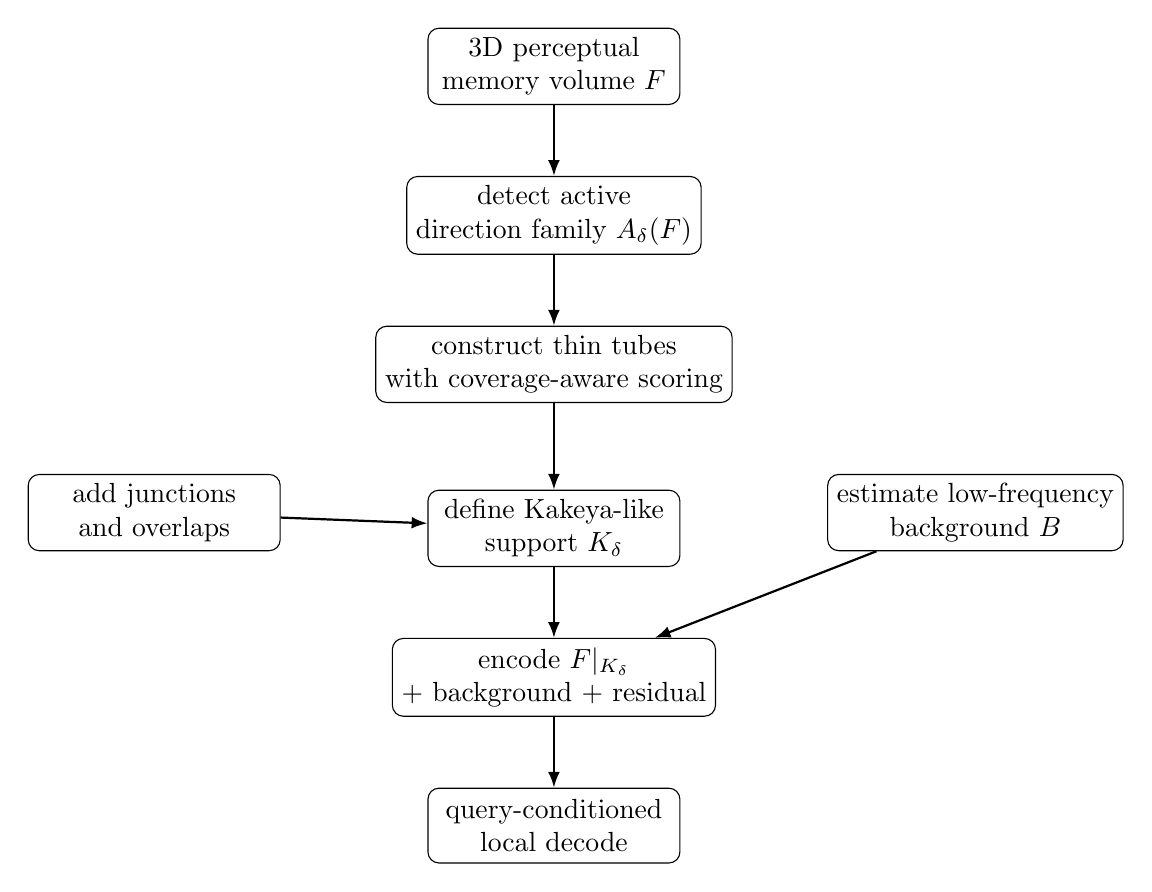
\begin{tikzpicture}[
    node distance=0.9cm and 0.8cm,
    box/.style={draw, rounded corners, align=center, minimum width=3.2cm, minimum height=0.95cm},
    arrow/.style={-{Latex[length=2mm]}, thick}
]
\node[box] (input) {3D perceptual\\memory volume $F$};
\node[box, below=of input] (dirs) {detect active\\direction family $A_\delta(F)$};
\node[box, below=of dirs] (tubes) {construct thin tubes\\with coverage-aware scoring};
\node[box, below left=of tubes, xshift=-0.4cm] (junctions) {add junctions\\and overlaps};
\node[box, below right=of tubes, xshift=0.4cm] (base) {estimate low-frequency\\background $B$};
\node[box, below=1.1cm of tubes] (support) {define Kakeya-like\\support $K_\delta$};
\node[box, below=of support] (encode) {encode $F|_{K_\delta}$\\+ background + residual};
\node[box, below=of encode] (query) {query-conditioned\\local decode};
\draw[arrow] (input) -- (dirs);
\draw[arrow] (dirs) -- (tubes);
\draw[arrow] (tubes) -- (support);
\draw[arrow] (junctions) -- (support);
\draw[arrow] (base) -- (encode);
\draw[arrow] (support) -- (encode);
\draw[arrow] (encode) -- (query);
\end{tikzpicture}
\caption{Support-first K3M pipeline. The key design choice is that the codec first constructs a thin Kakeya-like support $K_\delta$ and only then encodes the signal restricted to that support.}
\label{fig:k3m_pipeline}
\end{figure}

\section{K3M Coding Model}
Once the support is constructed, K3M encodes the signal through
\begin{equation}
\hat F = B + \sum_{m=1}^{M} a_m\psi_{T_m} + \sum_{n=1}^{N} b_n\phi_{J_n} + R.
\end{equation}
The interpretation is:
\begin{itemize}[leftmargin=1.5em]
\item $B$ is a low-frequency background,
\item $\psi_{T_m}$ are support-restricted tube signals,
\item $\phi_{J_n}$ are support-restricted junction signals,
\item $R$ is a residual outside or beyond the support model.
\end{itemize}

Crucially, this is not the primary definition of the method. It is \emph{secondary}. The primary definition is the construction of $K_\delta$.

\subsection{Where compression actually happens}
The codec is designed so that compression does \emph{not} primarily occur in a dense frequency table. It occurs in three layers:
\begin{enumerate}[leftmargin=1.5em]
\item \textbf{Support skeleton compression.} Only the support geometry is stored: tube endpoints, centerline control points or discrete line coordinates, direction labels, widths, modality tags, and temporal spans.
\item \textbf{Tube-signal compression.} Each tube stores only low-dimensional signal content along its centerline or local support coordinates, rather than a full ambient 3D block.
\item \textbf{Junction-structure compression.} Intersections, pivots, and overlaps are encoded explicitly so that multiple directions may reuse local support volume.
\end{enumerate}
This is the practical codec interpretation of the Kakeya-like principle: the support set is compressed first, the support-local signal second, and only a small residual remains outside this model.

\section{Mathematical Objective}
The core optimization target should be stated in the support-first form
\begin{align}
\min_{K_\delta,a,B}\quad
&\left\|F-B-\sum_{m=1}^{M} a_m \psi_{T_m}\right\|_2^2
+\lambda_1 |K_\delta|
+\lambda_2 C_{\mathrm{dir}}(K_\delta)
+\lambda_3 C_{\mathrm{attn}}(K_\delta)
+\lambda_4 \|R\|_{\mathrm{entropy}}.
\end{align}

Here:
\begin{itemize}[leftmargin=1.5em]
\item $B$ is the low-frequency background,
\item $\psi_{T_m}$ are atoms restricted to the tube supports,
\item $|K_\delta|$ is the support-volume penalty and is the Kakeya-critical term,
\item $C_{\mathrm{dir}}$ is a direction coverage constraint,
\item $C_{\mathrm{attn}}$ enforces usefulness for long-context attention,
\item $\|R\|_{\mathrm{entropy}}$ is the residual coding cost.
\end{itemize}

This formulation places support-volume minimization at the center of the codec and makes explicit that the principal compression objective is not only small reconstruction error, but a direction-rich representation supported on a very small set.

\begin{remark}
The conceptual correction in this paper is exactly that the second term,
\begin{equation}
\lambda_1 |K_\delta|,
\end{equation}
is not a minor regularizer attached to an otherwise standard codec. It is the term expressing the real compression value suggested by Kakeya-like geometry.
\end{remark}

\subsection{Prototype surrogate objective}
The current Python prototype does \emph{not} directly solve the support-first objective above. Instead, it uses a discrete greedy surrogate. First, it detects a finite active direction family. Then it incrementally constructs a support by selecting tubes with a coverage-aware score, adds junctions at overlap concentrations, and finally codes a sparse residual. This implementation should therefore be interpreted as a finite, engineering-oriented proxy for the main objective rather than a direct optimizer for it.

\begin{proposition}[Support-first memory decomposition]
Suppose a perceptual memory field $F$ admits a decomposition whose dominant directional content is concentrated near a discrete Kakeya-like support $K_\delta$. Then a support-first codec can be organized so that its total memory cost is controlled by three distinct terms:
\begin{equation}
\mathrm{Bits}(F)\approx \mathrm{Bits}(K_\delta)+\mathrm{Bits}(F|_{K_\delta})+\mathrm{Bits}(R),
\end{equation}
where $R$ is the residual not explained by the support model. Consequently, when the geometry of $K_\delta$ is substantially thinner than the ambient domain and the restriction $F|_{K_\delta}$ remains query-faithful, memory efficiency is governed more by support complexity than by ambient volume.
\end{proposition}

\begin{remark}
This proposition is intended as a design principle rather than a fully formal theorem. Its role is to state the paper's core claim in a theorem-like form: compression quality for long-context memory should be analyzed through support complexity, restricted signal complexity, and residual complexity, not only through dense rate-distortion.
\end{remark}

\subsection{Perceptual memory interpretation}
The intended memory interpretation of the decomposition is:
\begin{equation}
\mathrm{Memory} = \{\mathrm{Base},\ \mathrm{Tubes},\ \mathrm{JunctionGraph},\ \mathrm{Residual}\}.
\end{equation}
This structure is designed to mirror what long-horizon perceptual memory should preserve:
\begin{itemize}[leftmargin=1.5em]
\item \textbf{Tubes}: persistent motion trajectories, long-lived object cues, or topic continuation paths;
\item \textbf{JunctionGraph}: event pivots, crossings, merges, or transitions;
\item \textbf{Base}: stable background context;
\item \textbf{Residual}: fine details not captured by the support model.
\end{itemize}
Under this interpretation, memory storage is not ``the entire history volume,'' but a Kakeya-like memory skeleton together with restricted signal content on that skeleton.

\subsection{Full Memory-Oriented Objective}
The simplified support-first objective captures the main mechanism, but a fuller memory-oriented formulation is
\begin{equation}
\min_{B,T,J,R}
\mathcal{L}_{\mathrm{rec}}
+ \lambda_{\mathrm{vol}}\mathcal{L}_{\mathrm{vol}}
+ \lambda_{\mathrm{dir}}\mathcal{L}_{\mathrm{dir}}
+ \lambda_{\mathrm{junc}}\mathcal{L}_{\mathrm{junc}}
+ \lambda_{\mathrm{rate}}\mathcal{L}_{\mathrm{rate}}
+ \lambda_{\mathrm{attn}}\mathcal{L}_{\mathrm{attn}}
+ \lambda_{\mathrm{retr}}\mathcal{L}_{\mathrm{retr}}.
\end{equation}
Here the reconstruction term is
\begin{equation}
\mathcal{L}_{\mathrm{rec}}=\|F-\hat F\|_2^2,
\end{equation}
with
\begin{equation}
\hat F
=
B
+ \sum_{m=1}^{M} a_m\psi_{T_m}
+ \sum_{n=1}^{N} b_n\phi_{J_n}
+ R.
\end{equation}

The support-volume term is the operational Kakeya term:
\begin{equation}
\mathcal{L}_{\mathrm{vol}}=\mathrm{Vol}_\delta(K_\delta).
\end{equation}
In a discrete implementation, this may be replaced by a soft occupancy penalty of the form
\begin{equation}
\mathcal{L}_{\mathrm{vol}}
=
\sum_{x\in \Omega_\delta}
\left(
1-\exp\left(
-\sum_m M_m(x)-\sum_n N_n(x)-B_{\mathrm{mask}}(x)
\right)
\right),
\end{equation}
where $M_m(x)$ and $N_n(x)$ are soft occupancy masks for tubes and junctions.

The direction-coverage term prevents degenerate solutions that minimize volume by collapsing onto too few directions:
\begin{equation}
\mathcal{L}_{\mathrm{dir}}
=
\sum_{\theta\in A_\delta(F)}
\max\bigl(0,\eta-\mathrm{Cov}(\theta,K_\delta)\bigr),
\end{equation}
where $\mathrm{Cov}(\theta,K_\delta)$ measures how well the current support explains the active direction $\theta$.

The junction-complexity term encourages compact event structure while allowing necessary overlaps:
\begin{equation}
\mathcal{L}_{\mathrm{junc}}=\alpha |J| + \beta \sum_n \deg(J_n).
\end{equation}

The rate term decomposes by memory component:
\begin{equation}
\mathcal{L}_{\mathrm{rate}}
=
\mathrm{Bits}(B)+\mathrm{Bits}(T)+\mathrm{Bits}(J)+\mathrm{Bits}(R).
\end{equation}
This emphasizes that compression cost arises not only from residual coding, but also from the geometry and attributes of the support itself.

\subsection{Query-Faithful Attention and Retrieval Losses}
For long-context memory, reconstruction fidelity alone is insufficient. We therefore introduce query-faithfulness terms.

The first is an attention-preservation objective:
\begin{equation}
\mathcal{L}_{\mathrm{attn}}
=
\mathbb{E}_{q}
\left[
D\bigl(\mathrm{Attn}(F,q),\mathrm{Attn}(\hat F_q,q)\bigr)
\right],
\end{equation}
where $q$ is a query, $\hat F_q$ is the locally decoded memory under that query, and $D$ may be a KL divergence, an $\ell_2$ discrepancy, or a task-level mismatch.

The second is a retrieval-preservation objective:
\begin{equation}
\mathcal{L}_{\mathrm{retr}}
=
\mathbb{E}_{q}\left[1-\mathrm{Recall@}k(q;\mathrm{K3M})\right]
+
\mu\, \mathbb{E}_{q}\left[\mathrm{RankLoss}(q)\right].
\end{equation}
This term ensures that compressed memory remains searchable in a way that is consistent with downstream retrieval.

Together, these additions clarify that the intended notion of good compression in K3M is not merely dense replay quality. It is the preservation of query-conditioned usefulness under support-thin memory storage.

\section{Discrete Prototype Algorithm}
\subsection{Algorithmic steps}
The current prototype implements the following support-first pipeline:
\begin{enumerate}[leftmargin=1.5em]
\item Estimate a low-frequency background $B$ by separable box blur.
\item Compute the residual $E=F-B$.
\item On a finite direction bank, compute directional responses of $E$.
\item Greedily select a family of thin tubes with a direction-diversity penalty.
\item Form the discrete support $K_\delta$ as the union of the selected tubes.
\item Add junction neighborhoods at concentrated overlap sites.
\item Encode the tube-local signal, junction-local signal, and a sparse residual.
\item At query time, rank supports rather than the dense field.
\end{enumerate}

\subsection{Coverage-aware discrete scoring}
The present implementation makes the surrogate construction explicit by first detecting a small active direction family and then selecting tubes with a coverage-aware greedy score. For a candidate tube $T$ aligned with direction $\theta$, the discrete score is of the form
\begin{equation}
\mathrm{Score}(T)
\propto
\frac{\mathrm{Resp}(T)\cdot\bigl(1+\beta\,\mathbf{1}_{\theta\in U}\bigr)}
{(1+\gamma\,n_\theta)\,\mathrm{Vol}(T)^\alpha},
\end{equation}
where $\mathrm{Resp}(T)$ is the directional response, $U$ is the set of still-uncovered active directions, $n_\theta$ counts how often direction $\theta$ has already been selected, and $\mathrm{Vol}(T)$ is the discrete support volume of the candidate tube. This is not the main theoretical objective; it is the prototype-level surrogate used to approximately realize the support-volume-versus-direction-coverage tradeoff.

\subsection{Python alignment}
The present Python prototype in \texttt{k3m\_codec.py} is consistent with this corrected mechanism in the following precise sense:
\begin{itemize}[leftmargin=1.5em]
\item \texttt{encode()} first computes a background and residual, then constructs the support via tube selection and junction extraction, then encodes on that support.
\item \texttt{\_select\_tubes()} is the discrete Kakeya-like constructor: it scans a direction bank, measures directional response, and greedily adds support components.
\item \texttt{\_extract\_junctions()} adds overlap points, allowing local volume reuse between multiple directions.
\item \texttt{query\_decode()} reads memory by navigating the constructed support rather than scanning the entire dense tensor.
\end{itemize}

\paragraph{What the prototype does \emph{not} yet implement.}
It does not solve a global support optimization problem; instead it uses a greedy discrete approximation. It also does not construct a true minimal Kakeya set in the mathematical sense. The correct way to describe it is:
\begin{quote}
The current code is a coverage-aware discrete Kakeya-like support constructor, not a full optimal Kakeya support solver.
\end{quote}

\subsection{Query-Conditioned Decode}
K3M is intended to decode memory locally and conditionally rather than reconstructing the entire field. A query-conditioned read proceeds in four stages: query encoding, support retrieval, local support decoding, and local residual refinement. If $\mathcal{N}(q)$ denotes the query-selected support neighborhood, then the decoder produces
\begin{equation}
\hat F_q
=
\mathrm{DecodeBase}(q)
+
\mathrm{DecodeTubes}(\mathcal{N}(q))
+
\mathrm{DecodeJunctions}(\mathcal{N}(q))
+
\mathrm{DecodeResidual}(\mathcal{N}(q)).
\end{equation}
This makes explicit that K3M is a local-memory reconstruction mechanism. Its purpose is not to replay the full history volume, but to reconstruct the small support region most relevant to the current computation.

A schematic procedure is as follows:
\begin{enumerate}[leftmargin=1.5em]
\item encode the current query into a retrieval representation $q_{\mathrm{embed}}$,
\item retrieve a small set of seed junctions from the memory graph,
\item expand from those seed junctions to nearby or semantically aligned tubes under a budget,
\item decode only the base, tubes, junctions, and residual associated with that local support neighborhood.
\end{enumerate}
A more formal reference version of this procedure is given in Algorithm~\ref{alg:k3m-query-decode}.

\subsection{Memory-Graph Retrieval}
The junction structure naturally induces a memory graph. Junctions serve as graph nodes, and edges connect event pivots linked by shared tubes, temporal adjacency, topic continuation, causal hints, or cross-modal transitions. Retrieval is therefore organized over support geometry rather than dense volume.

This view is particularly useful for long-context attention. A transformer or downstream controller need not attend over the entire stored history. Instead, it may first attend coarsely over graph-level junction candidates, then expand to support-local tube content, and finally decode a small neighborhood around the chosen support. In this regime, the intended retrieval complexity is closer to
\begin{equation}
O(m_q + n_q + \mathrm{local\ decode\ cost}),
\end{equation}
where $m_q$ and $n_q$ are the numbers of retrieved tubes and junctions under query $q$, than to any complexity proportional to the full ambient volume.

\section{Related Work}
\subsection{Directional representation systems}
Curvelets and shearlets provide sparse representations for anisotropic structures. They are relevant because they show that directionality matters. However, they are still largely transform-centric. Our present emphasis is different: K3M is support-centric.

\subsection{Compression}
Classical and learned compression methods optimize rate-distortion on dense ambient signals. K3M instead asks whether support geometry can be thinned before full signal coding is attempted.

\subsection{Long-context memory}
Memory-augmented models, retrieval systems, and long-context architectures often compress history by chunking, summarizing, or indexing dense records. K3M offers a different substrate: a thin support set over which retrieval is organized.

\section{System Architecture for Perceptual Memory}
The conceptual contribution of K3M can be implemented as a practical long-context memory backend organized into six layers:
\begin{enumerate}[leftmargin=1.5em]
\item a Perceptual Lift Layer,
\item a Kakeya Support Constructor,
\item a Tube/Junction Encoder,
\item a Memory Graph Indexer,
\item a Query-Conditioned Decoder,
\item a Long-Context Attention Adapter.
\end{enumerate}
The purpose of this layered view is to separate modality-specific feature extraction from support construction, storage, and query-conditioned reconstruction.
Representative storage schemas and reference algorithms are collected in Appendix tables and algorithms; see Tables~\ref{tab:tuberecord-fields}--\ref{tab:attentionquery-fields} and Algorithms~\ref{alg:k3m-encode}--\ref{alg:k3m-query-decode}.

\subsection{Perceptual Lift Layer}
The Perceptual Lift Layer maps heterogeneous streams into a common memory field. For text, the input may include tokens, segment boundaries, speaker identity, and timestamps, which are mapped into a lifted field $F_{\mathrm{text}}(t,\mathrm{pos},\mathrm{sem})$. For images, one may use patch-level or region-level features, for example $F_{\mathrm{img}}(t,x,y)$ or $F_{\mathrm{img}}(t,\mathrm{patch},\mathrm{sem})$. For video, one may use frame sequences, patch trajectories, object slots, or motion cues, producing $F_{\mathrm{vid}}(t,x,y)$ or $F_{\mathrm{vid}}(t,\mathrm{patch},\mathrm{feature\text{-}group})$.

After lightweight cross-modal projection, the result is a unified memory tensor
\begin{equation}
F_{\mathrm{mem}} \in \mathbb{R}^{T\times U\times V\times C_0}.
\end{equation}
This unified tensor is the input to support construction.

\subsection{Kakeya Support Constructor}
The Kakeya Support Constructor is the core module. It is responsible for detecting active directions, proposing candidate tubes, selecting a support family, and identifying junctions. A practical implementation may be decomposed into four submodules:
\begin{enumerate}[leftmargin=1.5em]
\item a Direction Detector that estimates an active direction distribution on a finite bank,
\item a Tube Proposal Network that predicts candidate tubes with start point, end point, width, curvature, temporal extent, and modality tag,
\item a Support Selector that solves a sparse coverage problem balancing reconstruction, direction coverage, memory usefulness, and support volume,
\item a Junction Detector that extracts concentrated overlap points, high-curvature pivots, and residual hotspots.
\end{enumerate}
The present prototype instantiates this mechanism in a simplified form using a fixed direction bank and a greedy coverage-aware tube selector.

\subsection{Tube and Junction Encoding}
Each tube record stores support geometry together with a low-dimensional signal code. Typical tube attributes include a tube identifier, temporal span, direction label, centerline control points, radius, modality tag, semantic tag, importance score, and signal payload. The tube payload is not a dense 3D block. Instead, it stores a compact signal model in tube-local coordinates.

Each junction record stores a junction identifier, its location, the incident tube set, a junction type, an event or importance score, and a compact payload. Junction types may include merge, split, crossing, abrupt change, and semantic pivot.

The base component stores stable low-frequency structure such as persistent background context, long-lived scene configuration, or enduring topical state. The residual component stores details not captured by the base-plus-support model, potentially using a low-rate learned or classical entropy model.
Representative fields are summarized in Tables~\ref{tab:tuberecord-fields}, \ref{tab:junctionrecord-fields}, and \ref{tab:attentionquery-fields}.

\subsection{Memory Graph Indexing}
The memory graph organizes junctions as nodes and stores support-level relations as edges. Edge attributes may encode temporal adjacency, shared semantic topic, cross-modal bridge structure, coarse causal hints, or retrieval priors learned from data. This graph serves two purposes simultaneously: it is a compact index for memory search, and it is a structural prior for query expansion.

\subsection{Query-Conditioned Decoder}
The Query-Conditioned Decoder receives a query consisting of some combination of text prompt, modality filter, temporal constraint, entity set, topic set, and retrieval budget. It first retrieves seed junctions, then expands to a set of candidate tubes, then performs query-conditioned local decode on only those supports and their local neighborhoods. The output is a set of memory tokens or a local reconstructed fragment suitable for downstream reasoning.
Algorithm~\ref{alg:k3m-query-decode} gives a reference query-conditioned local decoding routine, while Table~\ref{tab:attentionquery-fields} summarizes a concrete structured query object.

\subsection{Long-Context Attention Adapter}
K3M can be coupled to a transformer in at least three ways. First, it may operate as an external memory backend, returning a small set of support-conditioned memory tokens for cross-attention. Second, it may support hierarchical attention, with coarse attention over junction tokens followed by fine attention over selected tube content. Third, in streaming settings, it may act as a tiered memory system in which the recent past remains dense, intermediate history is stored as tubes and junctions, and the distant past is retained only as base context, graph structure, and low-rate residual.

\subsection{Constraint-Edge Fixed as a Textual Support-First Proxy}
The current text-memory implementation used in our real-data experiments is not a full volumetric K3M codec. Instead, it should be understood as a support-first proxy architecture whose retrieval object is a discrete constraint-edge support rather than a dense token history. Concretely, the \texttt{constraint-edge fixed} pipeline:
\begin{enumerate}[leftmargin=1.5em]
\item extracts chunk-local state summaries and preferred/forbidden/required next-step signals,
\item maps them into a compact address-edge support with reusable junction-like overlaps,
\item ranks candidate sessions by a mixture of lexical cues and support overlap,
\item returns benchmark-native constraint objects, turning cues, and causal fragments from the selected support neighborhood.
\end{enumerate}

Philosophically, this matters because it matches the Kakeya-style inversion emphasized throughout the paper. The goal is not to preserve every token equally well. The goal is to preserve a thin structural support carrying the directions that matter for future recall: preference continuation, allowed/forbidden transitions, causal pivots, and turning points. In this textual setting, a ``direction'' is not a geometric line segment but a structured continuation constraint in memory space. The support archive therefore plays the role of a discrete Kakeya-like set: it is intentionally smaller than the full conversation trace, but still rich enough to cover multiple continuation directions under realistic user queries.

\subsection{Why a Mathematical Layer is Still Necessary Under LLM-Assisted Construction}
At first glance, one might think that if support construction is delegated to an LLM, then the mathematical layer becomes unnecessary. This is not the view of the present paper. The mathematical layer is still essential because it defines the \emph{object} that the LLM, heuristic extractor, or future learned model is supposed to construct.

The key distinction is between a \emph{construction mechanism} and a \emph{target structure}. An LLM may help propose states, continuations, pivots, or candidate support edges. But without a mathematical description of what counts as a valid support object, those outputs remain only free-form annotations. The role of the mathematical layer is to force these annotations to live in a constrained space:
\begin{enumerate}[leftmargin=1.5em]
\item a thin support should be preferred over a dense replay of the entire history,
\item the support should cover multiple future-useful directions,
\item the support should admit a compact archive representation,
\item query-time interaction should occur mainly through support geometry rather than full-history scanning.
\end{enumerate}

This is precisely why the notation around $K_\delta$, support ratio, junction structure, and support-restricted decoding is not decorative. It turns a prompt-generated summary into a memory object that can be compared, compressed, and evaluated.

There is also an implementation reason. The current best-performing PMS-Bench configuration, \texttt{constraint-edge fixed}, does not rely on online LLM interaction during the benchmark run; it uses an LLM-inspired schema together with a fallback local state-construction path. This would be impossible to interpret coherently if the project had no mathematical layer. The point of the formalism is to make LLM-assisted, heuristic, and future learned constructors interoperable by tying them to the same support-level abstraction.

In that sense, the mathematical layer answers a different question from the LLM. The LLM answers ``how might we propose a support?'' The mathematics answers ``what kind of object must that proposal become in order to count as a K3M memory support?'' The former can change with engineering practice; the latter is the real conceptual content of the method.

\section{Experimental Setup}
We evaluate K3M under two complementary empirical lenses.

\paragraph{Synthetic geometric validation.}
We first evaluate on synthetic $24\times24\times24$ volumes representing text-like, image-like, and multimodal memory structures. This benchmark compares K3M against:
\begin{enumerate}[leftmargin=1.5em]
\item \textbf{raw\_zlib},
\item \textbf{lowpass+sparse},
\item \textbf{wavelet-like}.
\end{enumerate}
For this setting we report compression ratio, relative $\ell_2$ error, PSNR, support ratio, and recall@3. The purpose of this experiment is geometric validation: does a support-first codec actually achieve thinner active support while preserving query usefulness?

\paragraph{Realistic memory evaluation.}
We then evaluate memory backends on real text-session benchmarks. Here the comparison is no longer between transform codecs, but between two kinds of memory realism:
\begin{enumerate}[leftmargin=1.5em]
\item \textbf{retrieval realism}, measured by the official AAAK retrieval path, which asks whether the system can recover the right session from a realistic haystack;
\item \textbf{perceptual-memory realism}, measured by PMS-Bench, which asks whether the system can recover user constraints, causal pivots, turning points, and cue-conditioned recall under compression.
\end{enumerate}

The PMS-Bench comparison in this paper uses official AAAK retrieval and the \texttt{constraint-edge fixed} support-first proxy described above. The latter uses query-guided constraint canonicalization, cue-aware reranking, and a real support-archive byte count. We report PMS score, retrieval and constraint subscores, recall@$k$, MRR, average raw bytes, average stored bytes, average compression ratio, support ratio, and query latency.

\section{Results}
\subsection{Synthetic geometric validation}
Table~\ref{tab:summary} reports average performance over the three synthetic datasets.

\begin{table}[t]
\centering
\caption{Average benchmark results on synthetic 3D memory volumes.}
\label{tab:summary}
\begin{tabular}{lcccccc}
\toprule
Method & Raw CR$\uparrow$ & zlib CR$\uparrow$ & Rel.\ $\ell_2\downarrow$ & PSNR$\uparrow$ & Support$\downarrow$ & Recall@3$\uparrow$ \\
\midrule
K3M & 1.84 & 1.68 & 0.2132 & 37.11 & 0.0596 & 0.89 \\
raw\_zlib & 1.09 & 1.00 & 0.0000 & 120.00 & 1.0000 & 0.89 \\
lowpass+sparse & 1.96 & 1.80 & 0.2472 & 35.79 & 1.0000 & 0.89 \\
wavelet-like & 6.94 & 6.35 & 0.1073 & 43.00 & 0.1991 & 0.89 \\
\bottomrule
\end{tabular}
\end{table}

The most important result is not that K3M has the best rate-distortion tradeoff; it does not. The decisive result is that it achieves the smallest support ratio while retaining the strongest average query recall achieved in the current benchmark. This is exactly the phenomenon that the corrected theory predicts should matter.

\begin{figure}[t]
\centering
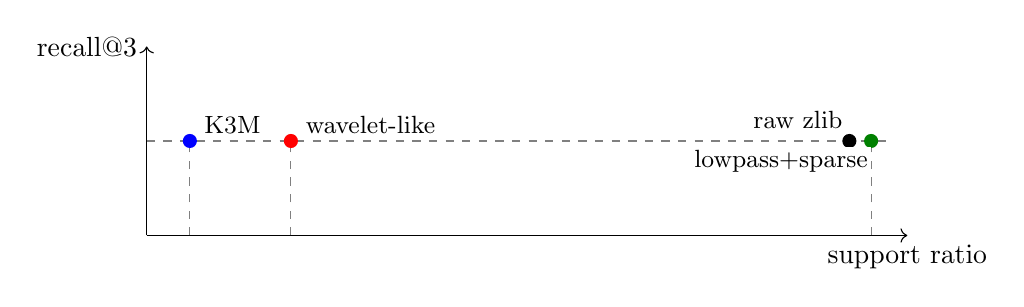
\begin{tikzpicture}[
    x=9.2cm,
    y=24cm,
    dot/.style={circle,fill,inner sep=1.8pt},
    lbl/.style={font=\small, fill=white, inner sep=1pt}
]
\draw[->] (0,0.84) -- (1.05,0.84) node[below] {support ratio};
\draw[->] (0,0.84) -- (0,0.94) node[left] {recall@3};

\draw[dashed,gray] (0.0596,0.84) -- (0.0596,0.89);
\draw[dashed,gray] (0.1991,0.84) -- (0.1991,0.89);
\draw[dashed,gray] (1.0,0.84) -- (1.0,0.89);
\draw[dashed,gray] (0,0.89) -- (1.02,0.89);

\node[dot,blue] at (0.0596,0.89) {};
\node[dot,red] at (0.1991,0.89) {};
\node[dot,green!50!black] at (1.0,0.89) {};
\node[dot,black] at (0.97,0.89) {};

\node[lbl,anchor=south west] at (0.075,0.892) {K3M};
\node[lbl,anchor=south west] at (0.215,0.892) {wavelet-like};
\node[lbl,anchor=south east] at (0.965,0.895) {raw zlib};
\node[lbl,anchor=north east] at (1.0,0.887) {lowpass+sparse};
\end{tikzpicture}
\caption{Support ratio versus recall@3. The main qualitative result is that K3M achieves the same average recall level as the strongest baselines in the current benchmark while operating on a substantially thinner active support.}
\label{fig:support_recall_tradeoff}
\end{figure}

\begin{figure}[t]
\centering
\begin{tikzpicture}[
    x=1.15cm,
    y=5.2cm,
    dot/.style={circle,fill,inner sep=1.8pt},
    lbl/.style={font=\small, fill=white, inner sep=1pt}
]
\draw[->] (0,0) -- (7.4,0) node[below] {raw compression ratio};
\draw[->] (0,0) -- (0,1.08) node[left] {support ratio};

\draw[dashed,gray] (1.84,0) -- (1.84,0.0596);
\draw[dashed,gray] (6.94,0) -- (6.94,0.1991);
\draw[dashed,gray] (1.96,0) -- (1.96,1.0);
\draw[dashed,gray] (1.09,0) -- (1.09,1.0);

\node[dot,blue] at (1.84,0.0596) {};
\node[dot,red] at (6.94,0.1991) {};
\node[dot,green!50!black] at (1.96,1.0) {};
\node[dot,black] at (1.09,1.0) {};

\node[lbl,anchor=south west] at (1.95,0.08) {K3M};
\node[lbl,anchor=south east] at (6.85,0.23) {wavelet-like};
\node[lbl,anchor=south west] at (2.05,0.98) {lowpass+sparse};
\node[lbl,anchor=south west] at (1.18,0.90) {raw zlib};
\end{tikzpicture}
\caption{Compression ratio versus support ratio. Wavelet-like coding is stronger on classical compression, but K3M occupies a much thinner active support. This illustrates the paper's central distinction between byte efficiency and support efficiency.}
\label{fig:compression_support_tradeoff}
\end{figure}

\subsection{Real-memory benchmark positioning}
Table~\ref{tab:pms-real-memory} reports the real-text memory comparison between official AAAK and \texttt{constraint-edge fixed} on PMS-Bench.

\begin{table}[t]
\centering
\caption{PMS-Bench comparison between official AAAK and the support-first \texttt{constraint-edge fixed} backend.}
\label{tab:pms-real-memory}
\resizebox{\textwidth}{!}{
\begin{tabular}{lcccccccc}
\toprule
Method & PMS$\uparrow$ & Retrieval$\uparrow$ & Constraint$\uparrow$ & Raw bytes & Stored bytes & Comp.\ $\uparrow$ & Support & Latency \\
\midrule
AAAK official & 0.4078 & 0.5639 & 0.0000 & 1209.0 & 81.2 & 14.89 & 0.0000 & 2991.69 ms \\
constraint-edge fixed & 0.7159 & 0.8858 & 1.0000 & 1458.8 & 366.1 & 3.98 & 0.5872 & 3.20 ms \\
\bottomrule
\end{tabular}
}
\end{table}

This table clarifies the main empirical point of the paper. Official AAAK is still the stronger pure compression-oriented retrieval system: it stores far fewer bytes per session than the current support-first proxy. However, once the task shifts from ``retrieve a relevant session'' to ``recover the user's structured memory state,'' the ordering reverses sharply. The support-first proxy wins on total PMS score, retrieval under the benchmark's own protocols, and benchmark-native constraint fidelity.

The strongest evidence for this claim is the constraint-recall slice. On PMS-Bench, official AAAK scores zero on allowed, forbidden, and required-set recovery, whereas \texttt{constraint-edge fixed} reaches perfect scores on all five constraint metrics in the current curated seed set. In other words, the support-first proxy is not merely returning vaguely related sessions; it is reconstructing the discrete continuation object that the benchmark asks the memory system to preserve.

\section{Discussion}
The benchmark suggests the following interpretation.

\paragraph{Compression ratio and support ratio are different quantities.}
Compression ratio measures stored bytes. Support ratio measures how much ambient memory remains active. The latter is the more direct reflection of the Kakeya-like principle.

\paragraph{A support-first codec may be worse on PSNR yet better for memory use.}
If the application is long-context retrieval rather than faithful dense replay, then a thinner support with high recall may be preferable to a denser but more distortion-efficient representation.

\paragraph{AAAK realism and PMS realism measure different user truths.}
The empirical tension between official AAAK and PMS-Bench is not a contradiction. It reflects two different notions of realism. AAAK is closer to the user environment in which the main challenge is broad haystack retrieval over heterogeneous session histories. PMS-Bench is closer to the user environment in which failure means misremembering preferences, violating stated boundaries, or missing a causal or turning-point update. The first is \emph{retrieval realism}; the second is \emph{perceptual-memory realism}. A practical long-term memory system should ideally perform well on both, but a support-first design is especially motivated by the second.

\paragraph{Why the Kakeya philosophy aligns more naturally with PMS-Bench.}
The Kakeya-style lesson in this paper is ``many directions, small volume.'' In a memory system, those directions correspond less to arbitrary semantic similarity and more to future-useful continuations: what the user now prefers, forbids, requires, or has pivoted toward. PMS-Bench measures whether those continuation directions survive compression. From this viewpoint, the benchmark is not an arbitrary custom metric suite. It is an operationalization of the paper's central philosophical claim that memory value lies in preserving thin, structurally meaningful supports rather than replaying dense history.

\paragraph{Why this helps long-context attention.}
The support-first architecture is useful precisely because long-context attention should not scale with the full ambient memory volume. Query-time reading is intended to proceed in stages:
\begin{enumerate}[leftmargin=1.5em]
\item find event-relevant junctions,
\item expand to the relevant tubes,
\item decode only a small neighborhood around those tubes,
\item perform fine attention on the resulting local memory fragment.
\end{enumerate}
Accordingly, the target retrieval complexity is not proportional to the total history volume, but closer in spirit to
\begin{equation}
O(\#\mathrm{relevant\ tubes} + \#\mathrm{relevant\ junctions}),
\end{equation}
up to the cost of local reconstruction. This is one of the main reasons to regard K3M as a memory backend rather than a generic transform codec.

\paragraph{The current prototype is conceptually aligned, but not yet numerically optimal.}
This is acceptable at the present stage because the goal of the project is to establish the correct mechanism first.

\section{Threats to Validity}
Several factors limit the scope of the current empirical claims.

\paragraph{Synthetic and real experiments still cover different abstractions.}
The synthetic benchmark validates the geometric mechanism of thin support construction, but it does not by itself prove utility on deployed agent memory. Conversely, PMS-Bench validates structured recall on real text sessions, but it still abstracts away from full multimodal streams and live user interaction loops. The current paper therefore establishes consistency across two partial lenses rather than a single definitive end-to-end benchmark.

\paragraph{Discrete proxy for continuous support construction.}
The current implementation uses a finite direction bank and a greedy support constructor. This is only a discrete approximation to the intended Kakeya-like mechanism, so the reported support ratios should be interpreted as proof-of-concept rather than sharp optima.

\paragraph{Task proxy mismatch.}
Recall@3 on synthetic volumes and PMS score on structured text memory are both proxies. They are useful because they isolate different parts of the support-first hypothesis, but neither is yet equivalent to downstream QA accuracy, planning performance, or long-context reasoning quality in a deployed assistant.

\paragraph{Baseline scope.}
The chosen baselines are deliberately simple and interpretable. They provide useful reference points, but they do not exhaust the space of modern compression or memory systems.

\section{Source Code Availability}
The submission artifact contains:
\begin{itemize}[leftmargin=1.5em]
\item \texttt{k3m\_codec.py},
\item \texttt{k3m\_benchmark.py},
\item this manuscript source.
\end{itemize}

\section{Practical Training Strategy}
A practical training pipeline for K3M is naturally staged.

In the first stage, modality-specific front ends are pretrained so that text, image, and video streams can be lifted into a roughly compatible memory space. In the second stage, the support-construction modules are trained to detect active directions, propose candidate tubes, and select thin supports with adequate directional coverage. In the third stage, the tube, junction, and residual codecs are trained for support-restricted reconstruction and rate control. In the fourth stage, the entire system is jointly tuned on downstream long-context tasks such as retrieval, question answering, multimodal reasoning, or agent memory usage.

This staged view is useful because support construction and query-faithful reconstruction are not identical objectives. The first is geometric and structural; the second is downstream and task-dependent.

\section{Evaluation Beyond Synthetic Compression}
The current synthetic benchmark is appropriate for validating the geometric mechanism of support-first compression, but a full evaluation of K3M should extend beyond classical rate-distortion metrics. The real-data results in this paper already suggest a two-axis evaluation template: retrieval realism on official haystack-style memory benchmarks, and perceptual-memory realism on benchmarks such as PMS-Bench that directly test constraints, pivots, and causal continuity. In addition to support ratio, compression ratio, relative reconstruction error, and recall@k, future evaluations should report long-context question answering accuracy, multimodal retrieval quality, query latency, decode-region size, memory bandwidth, and average numbers of active tubes and junctions per query.

An especially important next step is to evaluate whether K3M preserves useful reasoning trajectories under realistic query budgets. If the main application is long-context memory rather than dense replay, then support efficiency, retrieval quality, and budgeted decode fidelity may be more informative than PSNR alone.

\section{Limitations}
The current work has several limitations:
\begin{itemize}[leftmargin=1.5em]
\item the full volumetric K3M codec is still evaluated mainly on synthetic data,
\item the real-data support-first result uses a textual proxy architecture rather than the full 3D tube-and-junction codec,
\item the support constructor is greedy rather than globally optimized,
\item the direction bank is finite and hand-designed,
\item the tube geometry is straight rather than curved,
\item the entropy model is simple.
\end{itemize}

\section{Conclusion}
This paper rewrites the K3M project around what we regard as the correct core idea: the value of the three-dimensional Kakeya phenomenon for compression lies in constructing supports with high directional richness and very small volume.

K3M is therefore defined first as a support-construction mechanism and only second as a coding scheme. The current Python prototype is consistent with this corrected viewpoint at the level of a discrete greedy approximation. Its synthetic experiments already show the intended geometric behavior, and its support-first textual proxy shows that the same philosophy can outperform official AAAK on a benchmark aimed at perceptual-memory fidelity even while losing on pure compression ratio.

Our current conclusion is therefore deliberately two-part. If the target environment is broad haystack retrieval, official AAAK remains closer to the strongest current baseline. If the target environment is faithful long-term user memory---remembering constraints, pivots, and causal updates under compression---then a Kakeya-inspired support-first design appears substantially better aligned with the task. This is the benchmark-positioning claim of the paper: K3M should be judged not only by byte efficiency, but by whether a thin support can preserve the continuation structure that real users actually care about.

\appendix

\section{Implementation Consistency Check}
After rewriting the paper around Kakeya-like support construction, we re-checked the Python implementation against the corrected mechanism.

\paragraph{Consistent components.}
\begin{itemize}[leftmargin=1.5em]
\item The code constructs a support before final signal coding.
\item Tube selection is performed by active-direction detection followed by coverage-aware directional scanning over a fixed bank.
\item Junction extraction explicitly captures overlap reuse.
\item Query access is support-driven rather than full-volume scanning.
\end{itemize}

\paragraph{Current mismatches or simplifications.}
\begin{itemize}[leftmargin=1.5em]
\item The constructor is greedy, not globally optimal.
\item There is no explicit optimization enforcing a strict directional coverage constraint.
\item Background support is handled separately rather than as part of a unified minimal set construction.
\item The residual can still carry signal outside the thin support.
\end{itemize}

These are implementation simplifications, not conceptual contradictions. They should be presented as limitations of the current prototype.

\section{Reference Data Structures}
For completeness, we record a minimal engineering view of the memory package used by a K3M-style system. This appendix is not part of the conceptual definition of the codec, but it makes explicit how the support-first representation can be stored and queried in practice.

\paragraph{Memory package.}
A complete memory object may be written abstractly as
\begin{equation}
\begin{aligned}
\mathrm{MemoryPackage}
=
\{&\mathrm{BaseArchive},\ \mathrm{TubeRecords},\ \mathrm{JunctionRecords},\\
&\mathrm{MemoryGraph},\ \mathrm{ResidualArchive},\ \mathrm{Metadata}\}.
\end{aligned}
\end{equation}
Its intended role is to separate stable background content, support geometry, support-local signal payloads, graph structure, and residual detail.

\begin{definition}[TubeRecord]
A \emph{TubeRecord} is the stored representation of one support tube together with its support-local signal code. It contains a tube identifier, a temporal span $(t_0,t_1)$, a direction label or direction vector, centerline control points, a support radius, a modality tag, an optional semantic label, an importance score, a signal codec identifier, and a signal payload. The payload is not a dense ambient block; it stores a compact code in tube-local coordinates.
\end{definition}

\begin{table}[h]
\centering
\caption{Representative fields of a TubeRecord.}
\label{tab:tuberecord-fields}
\begin{tabular}{>{\raggedright\arraybackslash}p{0.26\textwidth} >{\raggedright\arraybackslash}p{0.64\textwidth}}
\toprule
Field & Description \\
\midrule
\texttt{tube\_id} & Unique identifier for the support tube. \\
\texttt{t\_0, t\_1} & Active temporal span of the tube. \\
\texttt{direction} & Dominant direction label or vector. \\
\texttt{control\_points} & Centerline control points or segment endpoints. \\
\texttt{radius} & Support radius or thickness parameter. \\
\texttt{modality} & Modality tag such as text, image, or video. \\
\texttt{semantic\_label} & Optional semantic or topical label. \\
\texttt{importance} & Retrieval or task-value score. \\
\texttt{signal\_codec} & Identifier of the local signal coding scheme. \\
\texttt{signal\_payload} & Tube-local compressed signal parameters. \\
\bottomrule
\end{tabular}
\end{table}

\begin{definition}[JunctionRecord]
A \emph{JunctionRecord} is the stored representation of one support junction. It contains a junction identifier, a location, the incident tube set, a junction type, an importance or event score, and a compact payload. Representative junction types include merge, split, crossing, abrupt change, and semantic pivot.
\end{definition}

\begin{table}[h]
\centering
\caption{Representative fields of a JunctionRecord.}
\label{tab:junctionrecord-fields}
\begin{tabular}{>{\raggedright\arraybackslash}p{0.26\textwidth} >{\raggedright\arraybackslash}p{0.64\textwidth}}
\toprule
Field & Description \\
\midrule
\texttt{junction\_id} & Unique identifier for the junction. \\
\texttt{location} & Junction location in the lifted memory domain. \\
\texttt{incident\_tubes} & Set or list of incident tube identifiers. \\
\texttt{junction\_type} & Structural role such as merge, split, crossing, or pivot. \\
\texttt{importance} & Event saliency or retrieval priority. \\
\texttt{payload} & Compact local signal or metadata payload. \\
\bottomrule
\end{tabular}
\end{table}

\paragraph{Memory graph.}
The graph view may be written abstractly as
\begin{equation}
\mathrm{MemoryGraph} = (\mathcal{V},\mathcal{E},\mathrm{Attr}),
\end{equation}
where $\mathcal{V}$ is the junction set, $\mathcal{E}$ contains adjacency relations induced by shared tubes or temporal continuity, and $\mathrm{Attr}$ stores edge-level annotations such as shared topic, temporal adjacency, causal hint, modality bridge, or retrieval prior.

\begin{definition}[AttentionQuery]
An \emph{AttentionQuery} is a structured retrieval request used to read from K3M under an explicit decode budget. It may contain an optional text query, a modality filter, an optional time range, entity constraints, topic constraints, and a retrieval or decode budget. This level of structure is useful because K3M is intended to return a budgeted local memory neighborhood rather than a replay of the full history volume.
\end{definition}

\begin{table}[h]
\centering
\caption{Representative fields of an AttentionQuery.}
\label{tab:attentionquery-fields}
\begin{tabular}{>{\raggedright\arraybackslash}p{0.26\textwidth} >{\raggedright\arraybackslash}p{0.64\textwidth}}
\toprule
Field & Description \\
\midrule
\texttt{text\_query} & Optional textual query or instruction. \\
\texttt{modality\_filter} & Allowed modalities for retrieval. \\
\texttt{time\_range} & Optional temporal restriction on the search. \\
\texttt{entities} & Entity-level constraints or anchors. \\
\texttt{topics} & Topic or semantic constraints. \\
\texttt{budget} & Maximum retrieval or local decode budget. \\
\bottomrule
\end{tabular}
\end{table}

\section{Reference Pseudocode}
We include schematic pseudocode to make the engineering pipeline explicit. These procedures are intended as readable reference implementations of the support-first idea, not as claims about the exact details of the current Python code.

\subsection{Encoding Procedure}
\begin{algorithm}[h]
\caption{Reference support-first K3M encoding procedure}
\label{alg:k3m-encode}
\begin{algorithmic}[1]
\Require Multimodal stream fragment $\mathcal{S}$; optional query prior $\pi_q$
\Ensure Encoded memory package $(\mathrm{quantB}, \mathrm{quantT}, \mathrm{quantJ}, \mathrm{memoryGraph}, \mathrm{quantR})$
\Procedure{EncodeK3M}{multimodal\_stream, query\_prior}
\State $F \gets \Call{PerceptualLift}{\text{multimodal\_stream}}$
\State $B \gets \Call{EstimateContextBase}{F}$
\State $E \gets F - B$
\State $\mathrm{activeDirs} \gets \Call{DetectActiveDirections}{E}$
\State $\mathrm{candidateTubes} \gets \Call{ProposeTubes}{E,\mathrm{activeDirs}}$
\State $\mathrm{selectedTubes} \gets \Call{SelectMinVolumeCover}{\mathrm{candidateTubes}, \text{objective}}$
\State $\mathrm{tubeCoeffs} \gets \Call{FitSignalsOnTubes}{E,\mathrm{selectedTubes}}$
\State $E_{\mathrm{tube}} \gets E - \Call{Synthesize}{\mathrm{selectedTubes},\mathrm{tubeCoeffs}}$
\State $\mathrm{candidateJunctions} \gets \Call{DetectJunctions}{\mathrm{selectedTubes},E_{\mathrm{tube}}}$
\State $\mathrm{selectedJunctions} \gets \Call{PruneJunctions}{\mathrm{candidateJunctions}}$
\State $\mathrm{junctionCoeffs} \gets \Call{FitSignalsOnJunctions}{E_{\mathrm{tube}},\mathrm{selectedJunctions}}$
\State $R \gets E_{\mathrm{tube}} - \Call{SynthesizeJunctions}{\mathrm{selectedJunctions},\mathrm{junctionCoeffs}}$
\State $\mathrm{quantB} \gets \Call{Quantize}{B}$
\State $\mathrm{quantT} \gets \Call{QuantizeTubes}{\mathrm{selectedTubes},\mathrm{tubeCoeffs}}$
\State $\mathrm{quantJ} \gets \Call{QuantizeJunctions}{\mathrm{selectedJunctions},\mathrm{junctionCoeffs}}$
\State $\mathrm{quantR} \gets \Call{EntropyCodeResidual}{R}$
\State $\mathrm{memoryGraph} \gets \Call{BuildJunctionGraph}{\mathrm{selectedTubes},\mathrm{selectedJunctions}}$
\State \Return $(\mathrm{quantB}, \mathrm{quantT}, \mathrm{quantJ}, \mathrm{memoryGraph}, \mathrm{quantR})$
\EndProcedure
\end{algorithmic}
\end{algorithm}
Algorithm~\ref{alg:k3m-encode} should be understood as an abstract pipeline specification rather than an exact implementation trace. If the support selector returns $M$ active tubes and $N$ active junctions, the dominant post-lifting cost is governed by candidate generation, support selection, local coefficient fitting, and residual coding. Abstractly, one may summarize the encode-side complexity as
\begin{equation}
O\bigl(C_{\mathrm{lift}} + C_{\mathrm{dir}} + C_{\mathrm{prop}} + C_{\mathrm{select}} + C_{\mathrm{fit}} + C_{\mathrm{entropy}}\bigr),
\end{equation}
where the individual terms denote, respectively, perceptual lifting, direction detection, proposal generation, support selection, support-local fitting, and entropy coding costs.

\subsection{Query-Conditioned Decoding Procedure}
\begin{algorithm}[h]
\caption{Reference query-conditioned K3M decoding procedure}
\label{alg:k3m-query-decode}
\begin{algorithmic}[1]
\Require Memory package $\mathcal{M}$; structured query $q$
\Ensure Local reconstructed memory fragment $\hat F_q$
\Procedure{QueryDecodeK3M}{memory, query}
\State $q_{\mathrm{embed}} \gets \Call{EncodeQuery}{\text{query}}$
\State $\mathrm{seedNodes} \gets \Call{RetrieveJunctions}{\text{memory.graph}, q_{\mathrm{embed}}}$
\State $\mathrm{candidateTubes} \gets \Call{ExpandFromGraph}{\text{memory.graph}, \mathrm{seedNodes}, q_{\mathrm{embed}}}$
\State $\mathrm{localBase} \gets \Call{DecodeBase}{\text{memory.base}, \text{query.timeSpan}}$
\State $\mathrm{localTubes} \gets \Call{DecodeTubes}{\text{memory.tubes}, \mathrm{candidateTubes}}$
\State $\mathrm{localJunctions} \gets \Call{DecodeJunctions}{\text{memory.junctions}, \mathrm{seedNodes}}$
\State $\mathrm{supportRegion} \gets \Call{Neighborhood}{\mathrm{candidateTubes}, \mathrm{seedNodes}}$
\State $\mathrm{localResidual} \gets \Call{DecodeResidual}{\text{memory.residual}, \mathrm{supportRegion}}$
\State $F_{\mathrm{local}} \gets \mathrm{localBase} + \mathrm{localTubes} + \mathrm{localJunctions} + \mathrm{localResidual}$
\State \Return $F_{\mathrm{local}}$
\EndProcedure
\end{algorithmic}
\end{algorithm}
If the query activates $m_q$ tubes and $n_q$ junctions, then the intended read-time complexity is closer to
\begin{equation}
O\bigl(C_{\mathrm{query}} + C_{\mathrm{retrieve}} + m_q + n_q + C_{\mathrm{local\ decode}}\bigr),
\end{equation}
than to any complexity proportional to the full ambient volume. This is the operational sense in which K3M seeks query-efficient long-context memory.

\subsection{Online Write and Offline Consolidation}
At the systems level, K3M may be operated in two complementary modes.

\paragraph{Online write path.}
\begin{enumerate}[leftmargin=1.5em]
\item receive a multimodal stream fragment,
\item lift it into $F_{\mathrm{mem}}$,
\item update a short-term dense cache,
\item detect active directions and saliency changes,
\item propose tube and junction candidates,
\item select a thin support increment,
\item encode base, tubes, junctions, and residual incrementally,
\item update the memory package and graph index.
\end{enumerate}

\paragraph{Offline consolidation path.}
\begin{enumerate}[leftmargin=1.5em]
\item merge redundant or nearly identical tubes,
\item merge nearby or semantically equivalent junctions,
\item reduce precision for low-importance supports,
\item further summarize distant residual content,
\item prune graph structure under storage or retrieval budgets.
\end{enumerate}
This separation is useful because the best write-time decision under a streaming constraint need not coincide with the best long-horizon storage decision after more context becomes available.

\begin{thebibliography}{9}
\bibitem{wolff1995}
T. Wolff.
\newblock An improved bound for Kakeya type maximal functions.
\newblock \emph{Revista Matem\'atica Iberoamericana}, 11(3):651--674, 1995.

\bibitem{dvir2009}
Z. Dvir.
\newblock On the size of Kakeya sets in finite fields.
\newblock \emph{Journal of the American Mathematical Society}, 22(4):1093--1097, 2009.

\bibitem{wangzahl2025}
H. Wang and J. Zahl.
\newblock Volume estimates for unions of convex sets, and the Kakeya set conjecture in three dimensions.
\newblock \emph{arXiv preprint arXiv:2502.17655}, 2025.
\newblock \url{https://arxiv.org/abs/2502.17655}.

\bibitem{candesdonoho2004}
E. Cand\`es and D. Donoho.
\newblock New tight frames of curvelets and optimal representations of objects with piecewise $C^2$ singularities.
\newblock \emph{Communications on Pure and Applied Mathematics}, 57(2):219--266, 2004.

\bibitem{kutynioklabate2012}
G. Kutyniok and D. Labate.
\newblock \emph{Shearlets: Multiscale Analysis for Multivariate Data}.
\newblock Birkh\"auser, 2012.

\bibitem{vaswani2017}
A. Vaswani et al.
\newblock Attention Is All You Need.
\newblock In \emph{Advances in Neural Information Processing Systems}, 2017.

\bibitem{balle2018}
J. Ball\'e, D. Minnen, S. Singh, S. J. Hwang, and N. Johnston.
\newblock Variational image compression with a scale hyperprior.
\newblock In \emph{International Conference on Learning Representations}, 2018.
\end{thebibliography}

\end{document}
